\documentclass{article}\usepackage[]{graphicx}\usepackage[]{color}
%% maxwidth is the original width if it is less than linewidth
%% otherwise use linewidth (to make sure the graphics do not exceed the margin)
\makeatletter
\def\maxwidth{ %
  \ifdim\Gin@nat@width>\linewidth
    \linewidth
  \else
    \Gin@nat@width
  \fi
}
\makeatother

\definecolor{fgcolor}{rgb}{0.345, 0.345, 0.345}
\newcommand{\hlnum}[1]{\textcolor[rgb]{0.686,0.059,0.569}{#1}}%
\newcommand{\hlstr}[1]{\textcolor[rgb]{0.192,0.494,0.8}{#1}}%
\newcommand{\hlcom}[1]{\textcolor[rgb]{0.678,0.584,0.686}{\textit{#1}}}%
\newcommand{\hlopt}[1]{\textcolor[rgb]{0,0,0}{#1}}%
\newcommand{\hlstd}[1]{\textcolor[rgb]{0.345,0.345,0.345}{#1}}%
\newcommand{\hlkwa}[1]{\textcolor[rgb]{0.161,0.373,0.58}{\textbf{#1}}}%
\newcommand{\hlkwb}[1]{\textcolor[rgb]{0.69,0.353,0.396}{#1}}%
\newcommand{\hlkwc}[1]{\textcolor[rgb]{0.333,0.667,0.333}{#1}}%
\newcommand{\hlkwd}[1]{\textcolor[rgb]{0.737,0.353,0.396}{\textbf{#1}}}%

\usepackage{framed}
\makeatletter
\newenvironment{kframe}{%
 \def\at@end@of@kframe{}%
 \ifinner\ifhmode%
  \def\at@end@of@kframe{\end{minipage}}%
  \begin{minipage}{\columnwidth}%
 \fi\fi%
 \def\FrameCommand##1{\hskip\@totalleftmargin \hskip-\fboxsep
 \colorbox{shadecolor}{##1}\hskip-\fboxsep
     % There is no \\@totalrightmargin, so:
     \hskip-\linewidth \hskip-\@totalleftmargin \hskip\columnwidth}%
 \MakeFramed {\advance\hsize-\width
   \@totalleftmargin\z@ \linewidth\hsize
   \@setminipage}}%
 {\par\unskip\endMakeFramed%
 \at@end@of@kframe}
\makeatother

\definecolor{shadecolor}{rgb}{.97, .97, .97}
\definecolor{messagecolor}{rgb}{0, 0, 0}
\definecolor{warningcolor}{rgb}{1, 0, 1}
\definecolor{errorcolor}{rgb}{1, 0, 0}
\newenvironment{knitrout}{}{} % an empty environment to be redefined in TeX

\usepackage{alltt}
\usepackage{geometry}
\usepackage{amsmath}
\usepackage{lscape}
\geometry{verbose,tmargin=2.5cm,bmargin=2.5cm,lmargin=2.5cm,rmargin=2.5cm}
\IfFileExists{upquote.sty}{\usepackage{upquote}}{}
\begin{document}



\begin{knitrout}
\definecolor{shadecolor}{rgb}{0.969, 0.969, 0.969}\color{fgcolor}\begin{kframe}
\begin{alltt}
\hlkwd{library}\hlstd{(survival)}
\end{alltt}


{\ttfamily\noindent\itshape\color{messagecolor}{\#\# Loading required package: splines}}\begin{alltt}
\hlkwd{load}\hlstd{(}\hlstr{"cpvs.20150119.RData"}\hlstd{)}

\hlkwd{sapply}\hlstd{(data.clin,} \hlkwa{function}\hlstd{(}\hlkwc{d}\hlstd{)} \hlkwd{c}\hlstd{(}\hlstr{"days_to_death"}\hlstd{,} \hlstr{"days_to_last_followup"}\hlstd{,} \hlstr{"vital_status"}\hlstd{)} \hlopt \hlkwd{colnames}\hlstd{(d))}
\end{alltt}
\begin{verbatim}
##       acc blca brca cesc coad dlbc esca  gbm hnsc kich kirc kirp laml  lgg
## [1,] TRUE TRUE TRUE TRUE TRUE TRUE TRUE TRUE TRUE TRUE TRUE TRUE TRUE TRUE
## [2,] TRUE TRUE TRUE TRUE TRUE TRUE TRUE TRUE TRUE TRUE TRUE TRUE TRUE TRUE
## [3,] TRUE TRUE TRUE TRUE TRUE TRUE TRUE TRUE TRUE TRUE TRUE TRUE TRUE TRUE
##      lihc luad lusc meso   ov paad prad read sarc skcm stad thca ucec  ucs
## [1,] TRUE TRUE TRUE TRUE TRUE TRUE TRUE TRUE TRUE TRUE TRUE TRUE TRUE TRUE
## [2,] TRUE TRUE TRUE TRUE TRUE TRUE TRUE TRUE TRUE TRUE TRUE TRUE TRUE TRUE
## [3,] TRUE TRUE TRUE TRUE TRUE TRUE TRUE TRUE TRUE TRUE TRUE TRUE TRUE TRUE
\end{verbatim}
\begin{alltt}
\hlstd{data.clin.merged} \hlkwb{=} \hlkwd{do.call}\hlstd{(rbind,} \hlkwd{lapply}\hlstd{(data.clin,} \hlkwa{function}\hlstd{(}\hlkwc{d}\hlstd{)} \hlkwd{apply}\hlstd{(d[,}\hlkwd{c}\hlstd{(}\hlstr{"bcr_patient_barcode"}\hlstd{,} \hlstr{"days_to_initial_pathologic_diagnosis"}\hlstd{,} \hlstr{"days_to_death"}\hlstd{,} \hlstr{"days_to_last_followup"}\hlstd{,} \hlstr{"vital_status"}\hlstd{)],} \hlnum{2}\hlstd{, as.character)))}
\hlstd{data.clin.merged} \hlkwb{=} \hlkwd{data.frame}\hlstd{(data.clin.merged,} \hlkwc{stringsAsFactors} \hlstd{=} \hlnum{FALSE}\hlstd{)}
\hlstd{data.clin.merged}\hlopt{$}\hlstd{days_to_death} \hlkwb{=} \hlkwd{as.numeric}\hlstd{(data.clin.merged}\hlopt{$}\hlstd{days_to_death)}
\end{alltt}


{\ttfamily\noindent\color{warningcolor}{\#\# Warning: NAs introduced by coercion}}\begin{alltt}
\hlstd{data.clin.merged}\hlopt{$}\hlstd{days_to_initial_pathologic_diagnosis} \hlkwb{=} \hlkwd{as.numeric}\hlstd{(data.clin.merged}\hlopt{$}\hlstd{days_to_initial_pathologic_diagnosis)}
\end{alltt}


{\ttfamily\noindent\color{warningcolor}{\#\# Warning: NAs introduced by coercion}}\begin{alltt}
\hlstd{data.clin.merged}\hlopt{$}\hlstd{days_to_last_followup} \hlkwb{=} \hlkwd{as.numeric}\hlstd{(data.clin.merged}\hlopt{$}\hlstd{days_to_last_followup)}
\end{alltt}


{\ttfamily\noindent\color{warningcolor}{\#\# Warning: NAs introduced by coercion}}\begin{alltt}
\hlstd{data.clin.merged}\hlopt{$}\hlstd{vital_status} \hlkwb{=} \hlkwd{as.factor}\hlstd{(data.clin.merged}\hlopt{$}\hlstd{vital_status)}
\hlstd{data.clin.merged}\hlopt{$}\hlstd{cancer} \hlkwb{=} \hlkwd{factor}\hlstd{(}\hlkwd{rep}\hlstd{(}\hlkwd{names}\hlstd{(data.clin),} \hlkwd{sapply}\hlstd{(data.clin, nrow)))}
\hlstd{data.clin.merged}\hlopt{$}\hlstd{event} \hlkwb{=} \hlstd{data.clin.merged}\hlopt{$}\hlstd{vital_status} \hlopt \hlkwd{c}\hlstd{(}\hlstr{"Dead"}\hlstd{,} \hlstr{"DECEASED"}\hlstd{)}

\hlstd{data.clin.merged}\hlopt{$}\hlstd{time} \hlkwb{=} \hlnum{NA}
\hlstd{data.clin.merged}\hlopt{$}\hlstd{time[data.clin.merged}\hlopt{$}\hlstd{event]} \hlkwb{=} \hlstd{data.clin.merged}\hlopt{$}\hlstd{days_to_death[data.clin.merged}\hlopt{$}\hlstd{event]} \hlopt{-} \hlstd{data.clin.merged}\hlopt{$}\hlstd{days_to_initial_pathologic_diagnosis[data.clin.merged}\hlopt{$}\hlstd{event]}
\hlstd{data.clin.merged}\hlopt{$}\hlstd{time[}\hlopt{!}\hlstd{data.clin.merged}\hlopt{$}\hlstd{event]} \hlkwb{=} \hlstd{data.clin.merged}\hlopt{$}\hlstd{days_to_last_followup[}\hlopt{!}\hlstd{data.clin.merged}\hlopt{$}\hlstd{event]} \hlopt{-} \hlstd{data.clin.merged}\hlopt{$}\hlstd{days_to_initial_pathologic_diagnosis[}\hlopt{!}\hlstd{data.clin.merged}\hlopt{$}\hlstd{event]}

\hlstd{data.clin.merged} \hlkwb{=} \hlstd{data.clin.merged[}\hlopt{!}\hlkwd{is.na}\hlstd{(data.clin.merged}\hlopt{$}\hlstd{time)} \hlopt{& !}\hlkwd{is.na}\hlstd{(data.clin.merged}\hlopt{$}\hlstd{event),]}

\hlkwd{library}\hlstd{(plyr)}
\hlstd{fits} \hlkwb{=} \hlkwd{dlply}\hlstd{(data.clin.merged,} \hlkwd{.}\hlstd{(cancer),} \hlkwa{function}\hlstd{(}\hlkwc{d}\hlstd{)} \hlkwd{survreg}\hlstd{(}\hlkwd{Surv}\hlstd{(d}\hlopt{$}\hlstd{time, d}\hlopt{$}\hlstd{event)} \hlopt{~} \hlnum{1}\hlstd{,} \hlkwc{dist} \hlstd{=} \hlstr{"logistic"}\hlstd{))}

\hlkwd{sort}\hlstd{(}\hlkwd{sapply}\hlstd{(fits,} \hlkwa{function}\hlstd{(}\hlkwc{f}\hlstd{) f}\hlopt{$}\hlstd{scale)} \hlopt{/} \hlkwd{sapply}\hlstd{(fits, coef))}
\end{alltt}
\begin{verbatim}
##   prad   thca   read   brca   ucec   kich   stad   kirp   dlbc    lgg 
## 0.1226 0.2120 0.2413 0.2717 0.2798 0.2890 0.2916 0.3026 0.3037 0.3223 
##   paad   coad   luad   kirc     ov   cesc   lihc   lusc   blca   sarc 
## 0.3249 0.3383 0.3519 0.3561 0.3612 0.3647 0.4011 0.4091 0.4259 0.4306 
##   esca   hnsc   skcm    acc    ucs    gbm   meso   laml 
## 0.4438 0.4445 0.4449 0.4507 0.5047 0.5162 0.6023 0.6408
\end{verbatim}
\begin{alltt}
\hlstd{rel_iqrs} \hlkwb{=} \hlkwd{dlply}\hlstd{(data.clin.merged,} \hlkwd{.}\hlstd{(cancer),} \hlkwa{function}\hlstd{(}\hlkwc{d}\hlstd{) \{}
        \hlstd{fit} \hlkwb{=} \hlkwd{survfit}\hlstd{(}\hlkwd{Surv}\hlstd{(d}\hlopt{$}\hlstd{time, d}\hlopt{$}\hlstd{event)} \hlopt{~} \hlnum{1}\hlstd{)}
        \hlstd{qs} \hlkwb{=} \hlkwd{approx}\hlstd{(fit}\hlopt{$}\hlstd{surv, fit}\hlopt{$}\hlstd{time,} \hlkwd{c}\hlstd{(}\hlnum{0.25}\hlstd{,} \hlnum{0.5}\hlstd{,} \hlnum{0.75}\hlstd{))}\hlopt{$}\hlstd{y}
        \hlstd{(qs[}\hlnum{1}\hlstd{]}\hlopt{-}\hlstd{qs[}\hlnum{3}\hlstd{])} \hlopt{/} \hlstd{qs[}\hlnum{2}\hlstd{]}
\hlstd{\})}

\hlkwd{sort}\hlstd{(}\hlkwd{unlist}\hlstd{(rel_iqrs))}
\end{alltt}
\begin{verbatim}
##   dlbc   paad     ov   stad    lgg    gbm   luad   lihc   skcm   lusc 
## 0.5399 0.8401 0.9979 1.0353 1.0976 1.1012 1.3945 1.5896 1.6648 1.6710 
##   hnsc    ucs   meso   laml 
## 1.7267 2.1334 2.8130 2.9566
\end{verbatim}
\begin{alltt}
\hlcom{# Right.  So PDAC is basically one of the most consistent cancers re: survival time.}
\hlcom{# Well there goes *that* argument.}
\end{alltt}
\end{kframe}
\end{knitrout}


\begin{knitrout}
\definecolor{shadecolor}{rgb}{0.969, 0.969, 0.969}\color{fgcolor}\begin{kframe}
\begin{alltt}
\hlcom{# Top 10 from AIHW2014:}
\hlcom{# Prostate (C61) 19,993}
\hlcom{# Colorectal (C18–C20) 15,151}
\hlcom{# Breast in females (C50) 14,465}
\hlcom{# Melanoma of the skin (C43) 11,570}
\hlcom{# Lung (C33–C34) 10,511}
\hlcom{# Non-Hodgkin lymphoma (C82–C85) 4,631}
\hlcom{# Kidney (C64) 2,847}
\hlcom{# Pancreas (C25) 2,748}
\hlcom{# Bladder (C67) 2,404}
\hlcom{# Uterus (C54–C55) 2,238}

\hlcom{# Stomach (C16) 2,093}

\hlkwd{library}\hlstd{(ggplot2)}
\end{alltt}


{\ttfamily\noindent\itshape\color{messagecolor}{\#\# Loading required package: methods}}\begin{alltt}
\hlkwd{library}\hlstd{(grid)}

\hlkwd{rm}\hlstd{(}\hlkwc{list} \hlstd{=} \hlkwd{ls}\hlstd{())}
\hlstd{cancer} \hlkwb{=}            \hlkwd{c}\hlstd{(}\hlstr{"Prostate"}\hlstd{,} \hlstr{"Colorectal"}\hlstd{,} \hlstr{"Breast"}\hlstd{,} \hlstr{"Melanoma"}\hlstd{,} \hlstr{"Lung"}\hlstd{,} \hlstr{"Non-Hodgkin Lymphoma"}\hlstd{,} \hlstr{"Kidney"}\hlstd{,}  \hlstr{"Pancreas"}\hlstd{,} \hlstr{"Bladder"}\hlstd{,} \hlstr{"Uterus"}\hlstd{)}
\hlstd{incidence_2011} \hlkwb{=}    \hlkwd{c}\hlstd{(}\hlnum{19993}\hlstd{,}      \hlnum{15151}\hlstd{,}        \hlnum{14465}\hlstd{,}    \hlnum{11570}\hlstd{,}      \hlnum{10511}\hlstd{,}  \hlnum{4631}\hlstd{,}                   \hlnum{2847}\hlstd{,}      \hlnum{2748}\hlstd{,}       \hlnum{2404}\hlstd{,}      \hlnum{2238}\hlstd{)}
\hlstd{survival_5yr_1982} \hlkwb{=} \hlkwd{c}\hlstd{(}\hlnum{58.2}\hlstd{,}       \hlnum{48.0}\hlstd{,}         \hlnum{71.9}\hlstd{,}     \hlnum{85.8}\hlstd{,}       \hlnum{8.7}\hlstd{,}    \hlnum{46.6}\hlstd{,}                   \hlnum{47.4}\hlstd{,}      \hlnum{3.0}\hlstd{,}        \hlnum{67.9}\hlstd{,}      \hlnum{74.7}\hlstd{)}
\hlstd{survival_5yr_2010} \hlkwb{=} \hlkwd{c}\hlstd{(}\hlnum{92.0}\hlstd{,}       \hlnum{66.2}\hlstd{,}         \hlnum{89.4}\hlstd{,}     \hlnum{90.7}\hlstd{,}       \hlnum{14.1}\hlstd{,}   \hlnum{70.6}\hlstd{,}                   \hlnum{71.9}\hlstd{,}      \hlnum{5.2}\hlstd{,}        \hlnum{57.5}\hlstd{,}      \hlnum{82.0}\hlstd{)}

\hlcom{# survival_historical = data.frame(cancer = rep(cancer, 2), incidence = rep(incidence_2011, 2), incidence_order = rep(order(incidence_2011), 2), time = rep(c("1982-1987", "2006-2010"), each = length(cancer)), surv = c(survival_5yr_1982, survival_5yr_2010))}
\hlstd{survival_historical} \hlkwb{=} \hlkwd{data.frame}\hlstd{(}\hlkwc{cancer} \hlstd{= cancer,} \hlkwc{incidence} \hlstd{= incidence_2011,} \hlkwc{incidence_rank} \hlstd{=} \hlkwd{rank}\hlstd{(incidence_2011),} \hlkwc{surv_rank} \hlstd{=} \hlkwd{rank}\hlstd{(survival_5yr_2010),} \hlkwc{surv1} \hlstd{= survival_5yr_1982,} \hlkwc{surv2} \hlstd{= survival_5yr_2010)}

\hlstd{survival_historical}\hlopt{$}\hlstd{cancer} \hlkwb{=} \hlkwd{ordered}\hlstd{(}\hlkwd{as.character}\hlstd{(survival_historical}\hlopt{$}\hlstd{cancer),} \hlkwc{levels} \hlstd{=} \hlkwd{as.character}\hlstd{(survival_historical}\hlopt{$}\hlstd{cancer)[}\hlkwd{order}\hlstd{(survival_historical}\hlopt{$}\hlstd{surv2)])}
\hlkwd{ggplot}\hlstd{(survival_historical,} \hlkwd{aes}\hlstd{(}\hlkwc{x} \hlstd{= cancer,} \hlkwc{xend} \hlstd{= cancer,} \hlkwc{y} \hlstd{= surv1,} \hlkwc{yend} \hlstd{= surv2))} \hlopt{+}
        \hlkwd{coord_flip}\hlstd{()} \hlopt{+}
        \hlkwd{geom_segment}\hlstd{(}\hlkwc{arrow} \hlstd{=} \hlkwd{arrow}\hlstd{(}\hlkwc{length} \hlstd{=} \hlkwd{unit}\hlstd{(}\hlnum{0.2}\hlstd{,} \hlstr{"cm"}\hlstd{),} \hlkwc{type} \hlstd{=} \hlstr{"closed"}\hlstd{),} \hlkwc{lwd} \hlstd{=} \hlnum{1.5}\hlstd{)} \hlopt{+}
        \hlkwd{ylab}\hlstd{(}\hlstr{"5 year survival (percent)"}\hlstd{)} \hlopt{+} \hlkwd{xlab}\hlstd{(}\hlstr{""}\hlstd{)} \hlopt{+} \hlkwd{theme_bw}\hlstd{()} \hlopt{+} \hlkwd{ylim}\hlstd{(}\hlnum{0}\hlstd{,} \hlnum{100}\hlstd{)} \hlopt{+}
        \hlkwd{annotate}\hlstd{(}\hlstr{"rect"}\hlstd{,} \hlkwc{xmin} \hlstd{=} \hlnum{0.85}\hlstd{,} \hlkwc{xmax} \hlstd{=} \hlnum{1.7}\hlstd{,} \hlkwc{ymin} \hlstd{=} \hlnum{55}\hlstd{,} \hlkwc{ymax} \hlstd{=} \hlnum{90}\hlstd{,} \hlkwc{fill} \hlstd{=} \hlstr{"white"}\hlstd{,} \hlkwc{colour} \hlstd{=} \hlstr{"grey"}\hlstd{,} \hlkwc{linetype} \hlstd{=} \hlstr{"solid"}\hlstd{)} \hlopt{+}
        \hlkwd{annotate}\hlstd{(}\hlstr{"segment"}\hlstd{,} \hlkwc{x} \hlstd{=} \hlnum{1.4}\hlstd{,} \hlkwc{xend} \hlstd{=} \hlnum{1.4}\hlstd{,} \hlkwc{y} \hlstd{=} \hlnum{65}\hlstd{,} \hlkwc{yend} \hlstd{=} \hlnum{80}\hlstd{,} \hlkwc{colour} \hlstd{=} \hlstr{"lightgrey"}\hlstd{,} \hlkwc{lwd} \hlstd{=} \hlnum{1.5}\hlstd{,} \hlkwc{arrow} \hlstd{=} \hlkwd{arrow}\hlstd{(}\hlkwc{length} \hlstd{=} \hlkwd{unit}\hlstd{(}\hlnum{0.2}\hlstd{,} \hlstr{"cm"}\hlstd{),} \hlkwc{type} \hlstd{=} \hlstr{"closed"}\hlstd{))} \hlopt{+}
        \hlkwd{annotate}\hlstd{(}\hlstr{"text"}\hlstd{,} \hlkwc{x} \hlstd{=} \hlnum{1.1}\hlstd{,} \hlkwc{y} \hlstd{=} \hlnum{65}\hlstd{,} \hlkwc{label} \hlstd{=} \hlstr{"1982-1987"}\hlstd{,} \hlkwc{cex} \hlstd{=} \hlnum{2.5}\hlstd{)} \hlopt{+}
        \hlkwd{annotate}\hlstd{(}\hlstr{"text"}\hlstd{,} \hlkwc{x} \hlstd{=} \hlnum{1.1}\hlstd{,} \hlkwc{y} \hlstd{=} \hlnum{80}\hlstd{,} \hlkwc{label} \hlstd{=} \hlstr{"2006-2010"}\hlstd{,} \hlkwc{cex} \hlstd{=} \hlnum{2.5}\hlstd{)}
\end{alltt}
\end{kframe}

{\centering 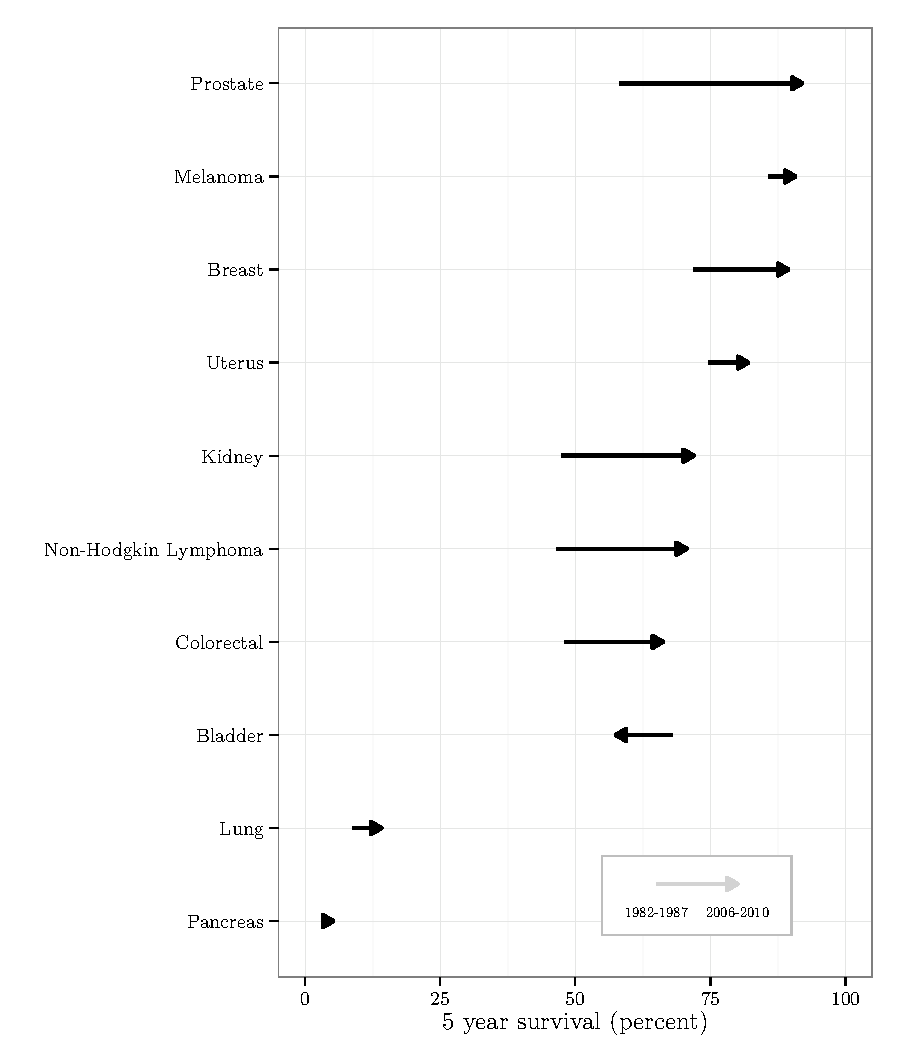
\includegraphics[width=\maxwidth]{figure/historical-survival-all-1} 

}


\begin{kframe}\begin{alltt}
\hlstd{survival_historical}\hlopt{$}\hlstd{cancer} \hlkwb{=} \hlkwd{ordered}\hlstd{(}\hlkwd{as.character}\hlstd{(survival_historical}\hlopt{$}\hlstd{cancer),} \hlkwc{levels} \hlstd{=} \hlkwd{as.character}\hlstd{(survival_historical}\hlopt{$}\hlstd{cancer)[}\hlkwd{order}\hlstd{(survival_historical}\hlopt{$}\hlstd{incidence)])}
\hlkwd{ggplot}\hlstd{(survival_historical,} \hlkwd{aes}\hlstd{(}\hlkwc{x} \hlstd{= cancer,} \hlkwc{xend} \hlstd{= cancer,} \hlkwc{y} \hlstd{= surv1,} \hlkwc{yend} \hlstd{= surv2))} \hlopt{+}
        \hlkwd{coord_flip}\hlstd{()} \hlopt{+}
        \hlkwd{geom_segment}\hlstd{(}\hlkwc{arrow} \hlstd{=} \hlkwd{arrow}\hlstd{(}\hlkwc{length} \hlstd{=} \hlkwd{unit}\hlstd{(}\hlnum{0.2}\hlstd{,} \hlstr{"cm"}\hlstd{),} \hlkwc{type} \hlstd{=} \hlstr{"closed"}\hlstd{),} \hlkwc{lwd} \hlstd{=} \hlnum{1.5}\hlstd{)} \hlopt{+}
        \hlkwd{ylab}\hlstd{(}\hlstr{"5 year survival (percent)"}\hlstd{)} \hlopt{+} \hlkwd{xlab}\hlstd{(}\hlstr{""}\hlstd{)} \hlopt{+} \hlkwd{theme_bw}\hlstd{()} \hlopt{+} \hlkwd{ylim}\hlstd{(}\hlnum{0}\hlstd{,} \hlnum{100}\hlstd{)}
\end{alltt}
\end{kframe}

{\centering 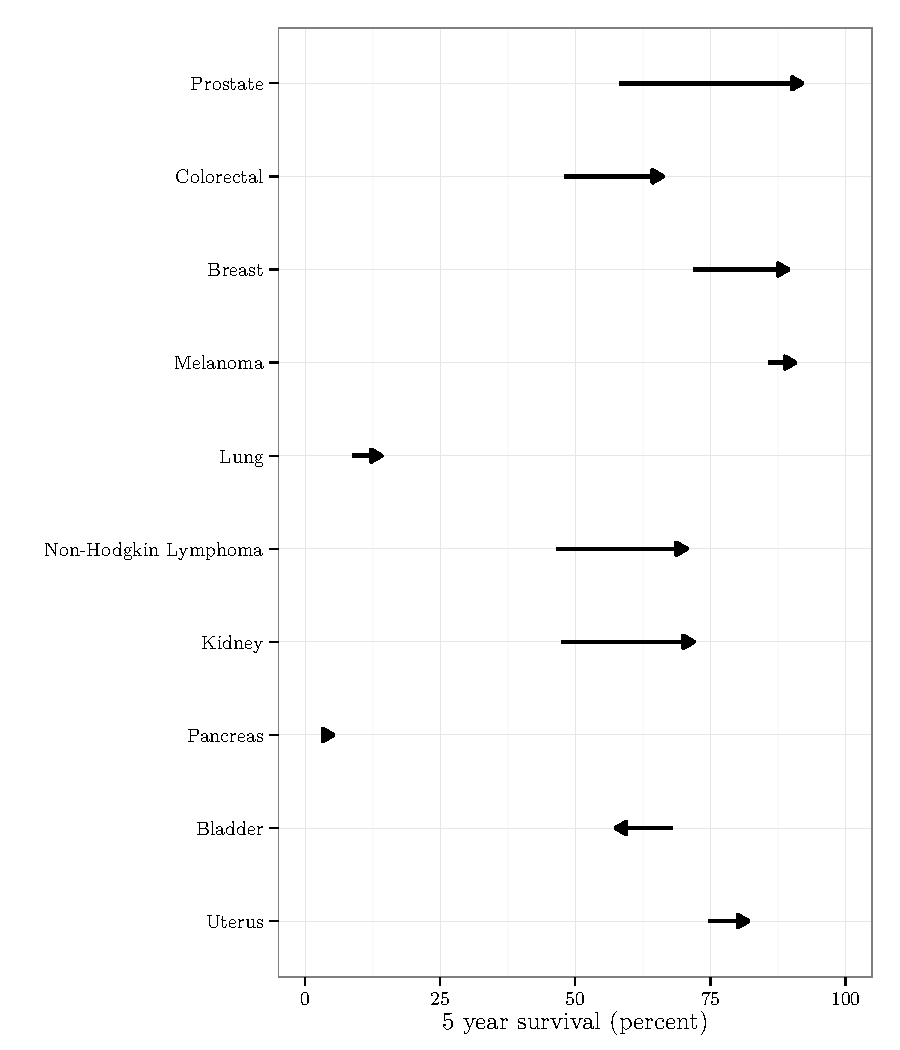
\includegraphics[width=\maxwidth]{figure/historical-survival-all-2} 

}



\end{knitrout}

\begin{knitrout}
\definecolor{shadecolor}{rgb}{0.969, 0.969, 0.969}\color{fgcolor}\begin{kframe}
\begin{alltt}
\hlcom{# Digitized data from AIHW2012:}
\hlstd{pdac_survival_5yr_aus_surv} \hlkwb{=} \hlkwd{c}\hlstd{(}\hlnum{4.55696}\hlstd{,} \hlnum{3.92405}\hlstd{,} \hlnum{3.41772}\hlstd{,} \hlnum{2.91139}\hlstd{,} \hlnum{2.53165}\hlstd{,} \hlnum{3.03797}\hlstd{,} \hlnum{3.29114}\hlstd{,} \hlnum{3.67089}\hlstd{,} \hlnum{3.67089}\hlstd{,} \hlnum{3.5443}\hlstd{,} \hlnum{3.41772}\hlstd{,} \hlnum{3.29114}\hlstd{,} \hlnum{3.16456}\hlstd{,} \hlnum{3.03797}\hlstd{,} \hlnum{2.91139}\hlstd{,} \hlnum{2.78481}\hlstd{,} \hlnum{3.03797}\hlstd{,} \hlnum{3.16456}\hlstd{,} \hlnum{3.41772}\hlstd{,} \hlnum{3.5443}\hlstd{,} \hlnum{3.5443}\hlstd{,} \hlnum{3.5443}\hlstd{,} \hlnum{3.5443}\hlstd{,} \hlnum{3.67089}\hlstd{,} \hlnum{3.67089}\hlstd{,} \hlnum{3.79747}\hlstd{,} \hlnum{3.79747}\hlstd{,} \hlnum{3.92405}\hlstd{,} \hlnum{4.05063}\hlstd{,} \hlnum{4.17722}\hlstd{,} \hlnum{4.17722}\hlstd{,} \hlnum{3.79747}\hlstd{,} \hlnum{3.5443}\hlstd{,} \hlnum{3.29114}\hlstd{,} \hlnum{3.5443}\hlstd{,} \hlnum{3.79747}\hlstd{,} \hlnum{4.05063}\hlstd{,} \hlnum{4.3038}\hlstd{,} \hlnum{4.3038}\hlstd{,} \hlnum{4.3038}\hlstd{,} \hlnum{4.17722}\hlstd{,} \hlnum{4.43038}\hlstd{,} \hlnum{4.55696}\hlstd{,} \hlnum{4.55696}\hlstd{,} \hlnum{4.81013}\hlstd{,} \hlnum{4.68354}\hlstd{,} \hlnum{4.68354}\hlstd{,} \hlnum{4.55696}\hlstd{,} \hlnum{4.55696}\hlstd{,} \hlnum{4.68354}\hlstd{,} \hlnum{4.68354}\hlstd{,} \hlnum{4.81013}\hlstd{,} \hlnum{4.81013}\hlstd{,} \hlnum{4.93671}\hlstd{,} \hlnum{5.18987}\hlstd{,} \hlnum{5.18987}\hlstd{,} \hlnum{5.18987}\hlstd{,} \hlnum{5.18987}\hlstd{,} \hlnum{5.18987}\hlstd{,} \hlnum{5.31646}\hlstd{,} \hlnum{5.18987}\hlstd{,} \hlnum{5.18987}\hlstd{,} \hlnum{5.31646}\hlstd{,} \hlnum{5.18987}\hlstd{,} \hlnum{5.18987}\hlstd{,} \hlnum{5.06329}\hlstd{,} \hlnum{5.06329}\hlstd{,} \hlnum{5.06329}\hlstd{,} \hlnum{4.93671}\hlstd{,} \hlnum{5.06329}\hlstd{,} \hlnum{4.93671}\hlstd{,} \hlnum{4.68354}\hlstd{,} \hlnum{4.43038}\hlstd{,} \hlnum{4.3038}\hlstd{,} \hlnum{4.3038}\hlstd{,} \hlnum{4.3038}\hlstd{,} \hlnum{4.17722}\hlstd{)}
\hlstd{pdac_survival_5yr_aus_yr} \hlkwb{=} \hlkwd{c}\hlstd{(}\hlnum{1985.996}\hlstd{,} \hlnum{1986.263}\hlstd{,} \hlnum{1986.53}\hlstd{,} \hlnum{1986.798}\hlstd{,} \hlnum{1987.065}\hlstd{,} \hlnum{1987.315}\hlstd{,} \hlnum{1987.6}\hlstd{,} \hlnum{1987.868}\hlstd{,} \hlnum{1988.135}\hlstd{,} \hlnum{1988.421}\hlstd{,} \hlnum{1988.688}\hlstd{,} \hlnum{1988.955}\hlstd{,} \hlnum{1989.241}\hlstd{,} \hlnum{1989.508}\hlstd{,} \hlnum{1989.776}\hlstd{,} \hlnum{1990.061}\hlstd{,} \hlnum{1990.328}\hlstd{,} \hlnum{1990.596}\hlstd{,} \hlnum{1990.881}\hlstd{,} \hlnum{1991.149}\hlstd{,} \hlnum{1991.416}\hlstd{,} \hlnum{1991.701}\hlstd{,} \hlnum{1991.969}\hlstd{,} \hlnum{1992.236}\hlstd{,} \hlnum{1992.522}\hlstd{,} \hlnum{1992.789}\hlstd{,} \hlnum{1993.056}\hlstd{,} \hlnum{1993.342}\hlstd{,} \hlnum{1993.609}\hlstd{,} \hlnum{1993.877}\hlstd{,} \hlnum{1994.162}\hlstd{,} \hlnum{1994.429}\hlstd{,} \hlnum{1994.697}\hlstd{,} \hlnum{1994.964}\hlstd{,} \hlnum{1995.232}\hlstd{,} \hlnum{1995.517}\hlstd{,} \hlnum{1995.785}\hlstd{,} \hlnum{1996.052}\hlstd{,} \hlnum{1996.337}\hlstd{,} \hlnum{1996.605}\hlstd{,} \hlnum{1996.872}\hlstd{,} \hlnum{1997.14}\hlstd{,} \hlnum{1997.425}\hlstd{,} \hlnum{1997.692}\hlstd{,} \hlnum{1997.96}\hlstd{,} \hlnum{1998.245}\hlstd{,} \hlnum{1998.513}\hlstd{,} \hlnum{1998.798}\hlstd{,} \hlnum{1999.065}\hlstd{,} \hlnum{1999.333}\hlstd{,} \hlnum{1999.618}\hlstd{,} \hlnum{1999.886}\hlstd{,} \hlnum{2000.153}\hlstd{,} \hlnum{2000.438}\hlstd{,} \hlnum{2000.706}\hlstd{,} \hlnum{2000.973}\hlstd{,} \hlnum{2001.259}\hlstd{,} \hlnum{2001.526}\hlstd{,} \hlnum{2001.811}\hlstd{,} \hlnum{2002.079}\hlstd{,} \hlnum{2002.346}\hlstd{,} \hlnum{2002.632}\hlstd{,} \hlnum{2002.899}\hlstd{,} \hlnum{2003.184}\hlstd{,} \hlnum{2003.452}\hlstd{,} \hlnum{2003.719}\hlstd{,} \hlnum{2004.004}\hlstd{,} \hlnum{2004.272}\hlstd{,} \hlnum{2004.539}\hlstd{,} \hlnum{2004.825}\hlstd{,} \hlnum{2005.092}\hlstd{,} \hlnum{2005.36}\hlstd{,} \hlnum{2005.645}\hlstd{,} \hlnum{2005.912}\hlstd{,} \hlnum{2006.18}\hlstd{,} \hlnum{2006.447}\hlstd{,} \hlnum{2006.733}\hlstd{)}
\hlstd{pdac_survival_5yr_aus_yr2} \hlkwb{=} \hlkwd{seq}\hlstd{(}\hlnum{1986}\hlstd{,} \hlnum{2007}\hlstd{,} \hlnum{3}\hlstd{)}
\hlstd{pdac_survival_5yr_aus_surv2} \hlkwb{=} \hlkwd{predict}\hlstd{(}\hlkwd{smooth.spline}\hlstd{(pdac_survival_5yr_aus_yr, pdac_survival_5yr_aus_surv,} \hlkwc{spar} \hlstd{=} \hlnum{0.75}\hlstd{), pdac_survival_5yr_aus_yr2)}\hlopt{$}\hlstd{y}
\hlkwd{plot}\hlstd{(pdac_survival_5yr_aus_surv} \hlopt{~} \hlstd{pdac_survival_5yr_aus_yr)}
\hlkwd{lines}\hlstd{(pdac_survival_5yr_aus_surv2} \hlopt{~} \hlstd{pdac_survival_5yr_aus_yr2)}
\end{alltt}
\end{kframe}

{\centering 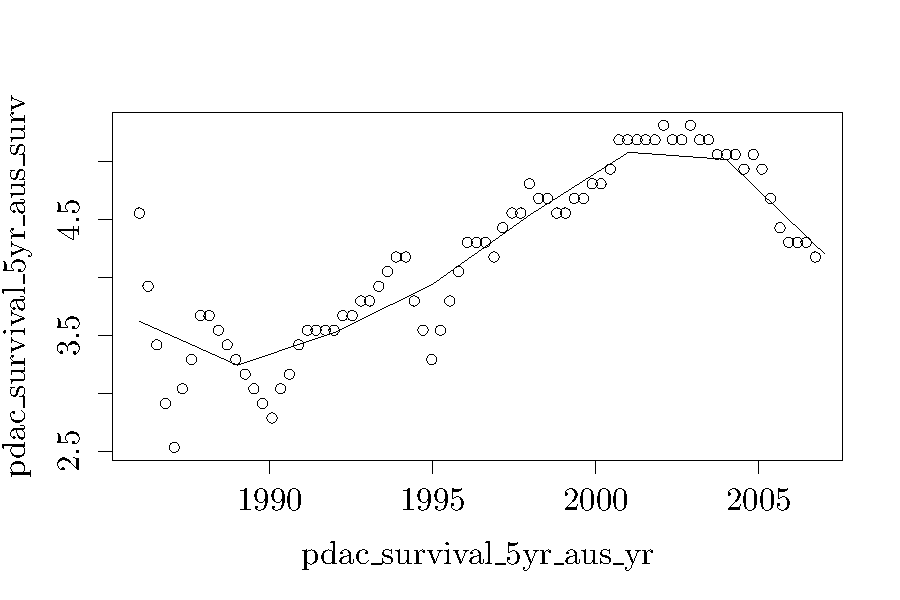
\includegraphics[width=\maxwidth]{figure/historical-survival-pdac-1} 

}


\begin{kframe}\begin{alltt}
\hlstd{pdac_survival_5yr_aus} \hlkwb{=} \hlkwd{data.frame}\hlstd{(}\hlkwc{Year} \hlstd{= pdac_survival_5yr_aus_yr2,} \hlkwc{Survival} \hlstd{= pdac_survival_5yr_aus_surv2)}

\hlcom{# Digitized data from NCI SEER:}
\hlstd{pdac_survival_5yr_usa_year} \hlkwb{=} \hlkwd{c}\hlstd{(}\hlkwd{seq}\hlstd{(}\hlnum{1976}\hlstd{,} \hlnum{1997}\hlstd{,} \hlnum{3}\hlstd{),} \hlnum{2001}\hlstd{,} \hlnum{2007}\hlstd{)}
\hlstd{pdac_survival_5yr_usa_surv} \hlkwb{=} \hlkwd{c}\hlstd{(}\hlnum{2.5}\hlstd{,} \hlnum{2.8}\hlstd{,} \hlnum{2.7}\hlstd{,} \hlnum{2.9}\hlstd{,} \hlnum{3.5}\hlstd{,} \hlnum{4.3}\hlstd{,} \hlnum{3.9}\hlstd{,} \hlnum{4.4}\hlstd{,} \hlnum{5.2}\hlstd{,} \hlnum{7.2}\hlstd{)}
\hlstd{pdac_survival_5yr_usa} \hlkwb{=} \hlkwd{data.frame}\hlstd{(}\hlkwc{Year} \hlstd{= pdac_survival_5yr_usa_year,} \hlkwc{Survival} \hlstd{= pdac_survival_5yr_usa_surv)}

\hlstd{pdac_survival_5yr} \hlkwb{=} \hlkwd{rbind}\hlstd{(}\hlkwd{cbind}\hlstd{(pdac_survival_5yr_aus,} \hlkwc{Country} \hlstd{=} \hlstr{"Australia"}\hlstd{),} \hlkwd{cbind}\hlstd{(pdac_survival_5yr_usa,} \hlkwc{Country} \hlstd{=} \hlstr{"USA"}\hlstd{))}
\hlkwd{ggplot}\hlstd{(pdac_survival_5yr,} \hlkwd{aes}\hlstd{(}\hlkwc{x} \hlstd{= Year,} \hlkwc{y} \hlstd{= Survival,} \hlkwc{colour} \hlstd{= Country))} \hlopt{+}
        \hlkwd{geom_line}\hlstd{(}\hlkwc{lwd} \hlstd{=} \hlnum{2}\hlstd{,} \hlkwc{alpha} \hlstd{=} \hlnum{0.5}\hlstd{)} \hlopt{+}
        \hlkwd{geom_point}\hlstd{(}\hlkwc{cex} \hlstd{=} \hlnum{4}\hlstd{)} \hlopt{+}
        \hlkwd{ylim}\hlstd{(}\hlnum{0}\hlstd{,} \hlnum{10}\hlstd{)} \hlopt{+}
        \hlkwd{theme_bw}\hlstd{()} \hlopt{+}
        \hlkwd{geom_segment}\hlstd{(}\hlkwc{x} \hlstd{=} \hlnum{1997}\hlstd{,} \hlkwc{xend} \hlstd{=} \hlnum{1997}\hlstd{,} \hlkwc{y} \hlstd{=} \hlnum{5.5}\hlstd{,} \hlkwc{yend} \hlstd{=} \hlnum{5}\hlstd{,} \hlkwc{colour} \hlstd{=} \hlstr{"#fc8d62"}\hlstd{,} \hlkwc{alpha} \hlstd{=} \hlnum{0.5}\hlstd{,} \hlkwc{lwd} \hlstd{=} \hlnum{1.5}\hlstd{,} \hlkwc{arrow} \hlstd{=} \hlkwd{arrow}\hlstd{(}\hlkwc{length} \hlstd{=} \hlkwd{unit}\hlstd{(}\hlnum{0.2}\hlstd{,} \hlstr{"cm"}\hlstd{)))} \hlopt{+}
        \hlkwd{geom_segment}\hlstd{(}\hlkwc{x} \hlstd{=} \hlnum{2007}\hlstd{,} \hlkwc{xend} \hlstd{=} \hlnum{2007}\hlstd{,} \hlkwc{y} \hlstd{=} \hlnum{3}\hlstd{,} \hlkwc{yend} \hlstd{=} \hlnum{3.5}\hlstd{,} \hlkwc{colour} \hlstd{=} \hlstr{"#66c2a5"}\hlstd{,} \hlkwc{alpha} \hlstd{=} \hlnum{0.5}\hlstd{,} \hlkwc{lwd} \hlstd{=} \hlnum{1.5}\hlstd{,} \hlkwc{arrow} \hlstd{=} \hlkwd{arrow}\hlstd{(}\hlkwc{length} \hlstd{=} \hlkwd{unit}\hlstd{(}\hlnum{0.2}\hlstd{,} \hlstr{"cm"}\hlstd{)))} \hlopt{+}
        \hlkwd{ylab}\hlstd{(}\hlstr{"5-year survival (percent)"}\hlstd{)} \hlopt{+}
        \hlkwd{scale_colour_brewer}\hlstd{(}\hlkwc{palette} \hlstd{=} \hlstr{"Set2"}\hlstd{)}
\end{alltt}
\end{kframe}

{\centering 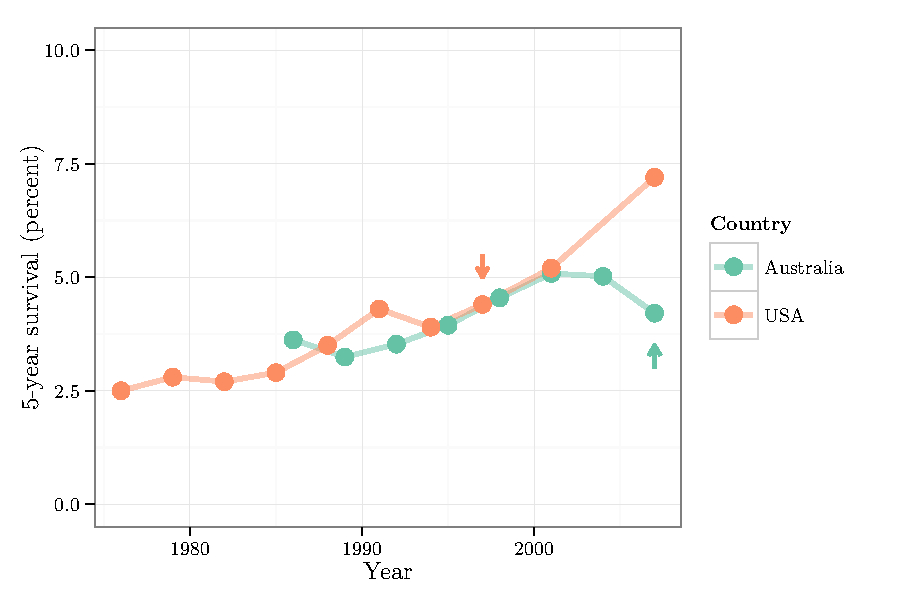
\includegraphics[width=\maxwidth]{figure/historical-survival-pdac-2} 

}


\begin{kframe}\begin{alltt}
\hlcom{# Surgery (adjuvant): Gemcitabine / 5-FU / capecitabine (w/ or w/o radio)}
\hlcom{# Metastatic: FOLFIRINOX / Gem-nabpac / Gem-erlotinib / gem / 5-FU}

\hlcom{# FOLFIRINOX 2010}
\hlcom{# Gem 1996 (UK) - 1997 (USA) - 2007 (Aus)}
\end{alltt}
\end{kframe}
\end{knitrout}

\end{document}
